\documentclass[final]{beamer}
\mode<presentation>
{
   \usetheme{AlabamaPoster}
}
\usepackage{times}
\usepackage[english]{babel}
\usepackage[latin1]{inputenc}
%\usepackage[orientation=landscape,size=a0,scale=1.4,debug]{beamerposter}
\usepackage[orientation=landscape,size=a0,scale=1.55,debug]{beamerposter}
%\usepackage[orientation=landscape,size=custom,width=27.5,height=21.5,scale=0.3]{beamerposter}
\usepackage{array}
\usepackage{comment}
\usepackage{ragged2e}
\usepackage{booktabs}   % provides \toprule, \midrule, \bottomrule (varying thicknesses)
\usepackage{multirow}
\usepackage{url} 
\usepackage{listings}
\usepackage{float}
\usepackage{wrapfig}
\usepackage{verbatim}



\graphicspath{{graphics/}}

\title{Automatic Recovery of Impacted Method Sets from Resolved Bug Reports}
\author[Corley]{Corley}
\institute[The University of Alabama]{Department of Computer Science, The University of Alabama}
\date{\today}

\begin{document}
\begin{frame}{}
    \begin{columns}[t]
        \begin{column}{.32\linewidth}


            \begin{block}{\large\sc Abstract}
                \vspace*{-0.25em}
                \centering
                \begin{minipage}[t]{0.95\linewidth}
\justifying
\large
Open source software development teams often use a revision control system,
such as CVS, and a bug tracking system, such as Bugzilla, to manage software
evolution tasks.
Utilizing patch data retrieved from resolved Bugzilla bug reports, impacted method sets in source code can be extracted.
\vskip0.5\baselineskip
In the past, manual inspection of the patch was required to recover the impacted methods; however, this is a time consuming process.
Our tool uses an automated approach to recover impacted method sets from resolved bug reports.
                \end{minipage}
                \vspace*{-0.5em}
            \end{block}


            \begin{block}{\large\sc Patch File}
                \vspace*{-0.25em}
                \centering
                \begin{minipage}[t]{0.95\linewidth}
\large
\justifying
A patch file contains data which describes the differences between two sets of files.  The comparison of files is done line by line.
In software development, patches are used to list the changes between old source code and new source code.
Applying a patch file will bring any unchanged files up to date.
Bug tracking systems allow users to submit patches as solutions to bug reports.\\
\vskip0.22\baselineskip
\centering
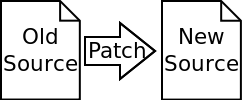
\includegraphics[width=10em]{patch}\\
\justifying
Patches contain much usable data:
\begin{itemize}
\item
    File names of old and new sources
\item
    Dates of last changes to each source
\item
    Line ranges where changes occur
\item
    Context lines that were unchanged
\item
    Each line change with special denotation
\end{itemize}

                \end{minipage}
                \vspace*{-0.5em}
            \end{block}
        \end{column}


        \begin{column}{.66\linewidth}
            \begin{block}{\large\sc Methodology}
                \vspace*{-0.25em}
                \centering
                \begin{minipage}[t]{0.975\linewidth}
\centering
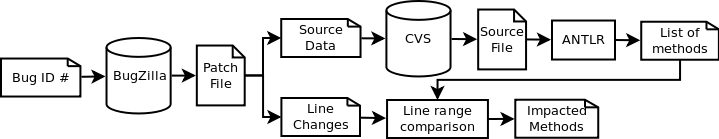
\includegraphics[width=\linewidth]{processwider}
\large
\justifying
%Our methodology for completing the task for patch file analysis can be seen in the above figure.
%A summary of the actions taken to complete this task are as follows:
%\begin{enumerate}
%\item
%    Obtain information related to bug from Bugzilla, specifically the patch file
%\item
%    Detect which source files are changed by the patch
%\item
%    Retrieve the correct revision of each original source file from CVS
%\item
%    Parse the original source file using ANTLR, in which our grammar builds a list of method objects
%\item
%    In the patch, detect which line numbers have differences from the source
%\item
%    A changed method will have a line range including one of line numbers
%\end{enumerate}
%\vskip0.95\baselineskip

                \end{minipage}
                \vspace*{0.46em}
            \end{block}


            \begin{block}{\large\sc Experiments}
                \vspace*{-0.25em}
                \centering
                \begin{minipage}[t]{0.975\linewidth}
\vspace*{-1em}
\justifying
\large
\begin{wrapfigure}{r}{0.57\linewidth}
\vskip0.5em
\hskip1em
\begin{tabular}{|l|rrrrr|}
\hline
\multirow{2}{*}{Software} & Manual & Automatic & \multirow{2}{*}{Agreed} & \multirow{2}{*}{Disagreed} & Task \\
& Results & Results & & & Mismatch  \\
\hline
Rhino   & 655  & 866  & 600  & 242  & 79  \\
Eclipse & 953  & 1938 & 847  & 461  & 736 \\
\hline
Total   & 1608 & 2804 & 1447 & 703  & 815 \\
\hline
\end{tabular}
\caption{Number of impacted methods}
\end{wrapfigure}

In order to test the accuracy of our methodology, we performed case studies on two software projects.
Our goal was to measure our automatic approach in comparison to manual inspection.  
Our data set consists of resolved Bugzilla bug reports for Mozilla Rhino and Eclipse.
We considered 104 Rhino bug reports and 203 Eclipse bug reports.
\vskip0.5\baselineskip
%\begin{wrapfigure}{r}{0.2\linewidth}
%\centering
%\vskip-2em
%\includegraphics[width=\linewidth]{venn}
%\end{wrapfigure}
Comparing results between manual and automatic inspection, both agreements and disagreements in which methods were changed were found.
%Agreements are represented by section A of the Venn diagram, while sections B and C represent disagreements.
%Of the 703 methods in disagreement, our automatic approach was incorrect for 24 (section B).  These can be classified in one of the following categories:
Of the 703 methods in disagreement, our automatic approach was incorrect for 24.  These can be classified in one of the following categories:
\vskip0.1\baselineskip
\begin{itemize}
\item
    Changes outside method body range
    \begin{itemize}
    \justifying
    \large
    \item
        Lines in the global scope of the class
    \item
        Lines on or after the original method's ending brace (exclusive range)
    \end{itemize}
\item
    Fixes for files that do not appear in any milestone releases we inspected
\item
    Patches embedded in bug report comments which were corrupted
\end{itemize}
    
                \end{minipage}
                \vspace*{-0.5em}
            \end{block}

            \vspace*{-1.25em}
            \begin{column}{.49\linewidth}
                \begin{block}{\large\sc Applications}
                    \vspace*{-0.25em}
                    \centering
                    \begin{minipage}[t]{0.95\linewidth}
\justifying
\large
Impacted method sets are utilized in many areas:
\begin{itemize}
\item
    Fault prediction models
\item
    Bug localization
\item
    Concept location
%\item
%    Patch analysis
\end{itemize}


                    \end{minipage}
                    \vspace*{-0.5em}
                \end{block}
            \end{column}
            \begin{column}{.49\linewidth}
                \begin{block}{\large\sc Acknowledgments}
                    \vspace*{-0.25em}
                    \begin{minipage}[t]{0.7\linewidth}
                        \vspace*{-5.75em}
\justifying
\large
The work presented in this poster is supported in part by the National Science Foundation under Grant No. 0851824.
                    \end{minipage}
                    \hskip2ex
                    \begin{minipage}[t]{0.22\linewidth}
\centering

\includegraphics[width=\linewidth]{NSF}
                    \end{minipage}
                    \vspace*{-1.715em}
                \end{block}
            \end{column}


        \end{column}
    \end{columns}
\vspace*{-.2em}
\end{frame}
\end{document}

% vim:syntax=tex
